\documentclass[a4,12pt]{scrartcl}

%Basic 
\usepackage[utf8]{inputenc}
\usepackage[ngerman]{babel}
\usepackage[T1]{fontenc}
%Schrift 
\usepackage{textcomp} % Für μ \textmu
%\usepackage{fontspec} 
%\setmainfont{Arial} 
%Zeilenabstand
\usepackage{setspace}
\setstretch {1.3}
\usepackage{float}
\usepackage[bottom = 3.50cm]{geometry}

%Titel Seite
\usepackage{titling} %Wird benötigt damit \maketitle die Variabeln title, author und date nicht überschreibt
\title{Schlussbericht}
\subtitle{Projekt: sniffdatel}
\author{David Meister \and Giorgio Vincenti \and Samuel Krieg \and Andreas Stalder}		
 %mit /and können Personen hinzugefügt werden
\date{\today}


%Kopf, Fusszeile
\usepackage{fancyhdr}
\pagestyle{fancy}
\lhead{SW Engineering Projekt FS 2016}
\chead{}
\rhead{sniffdatel}
\lfoot{\thetitle \: v1.0 }
\cfoot{\today }
\rfoot{Seite \thepage}
\renewcommand{\headrulewidth}{0.4pt}

%Bilder
\usepackage{graphicx}

%Zeichnen
\usepackage{tikz}

%Tabellen
\usepackage{booktabs}
\usepackage{longtable}

%Codesnippets
\usepackage{listings}
\lstset{language=java,basicstyle=\footnotesize,frame=single} %backgroundcolor=\color{lightgray}

%Querformat für eine Seite
\usepackage{lscape}
\usepackage{rotating}
\usepackage{pdflscape}

%URL 
\usepackage[colorlinks=true, linkcolor=blue, urlcolor=blue, citecolor=blue]{hyperref}
\urlstyle{same} 


%Loremimpsum
\usepackage{lipsum}



\begin{document}

%\clearpage\maketitle
\begin{titlepage}
	\centering
	\vspace{5cm}
	\begin{center}
	
\includegraphics[width=0.50\textwidth]{logo.png}
	\end{center}
	{\huge\bfseries sniffdatel\par}
	\vspace{8cm}
	\raggedright
	{\bfseries SW Engineering Projekt FS 2016\par}
	{\huge\bfseries Schlussbericht\par}
	\vspace{1cm}
	{\theauthor \par}
	{\today\par}

\end{titlepage}

\section{Änderungsgeschichte}

\begin{table}[htb]
\centering
    \begin{tabular}{@{} l l l l@{}}\toprule    
    {Datum} & {Version} & {Änderung} & {Autor}\\ \midrule
    26.05.16 & 1.0 & Erstellung erster Version & Giorgio Vincenti\\ \addlinespace
    31.05.16 & 1.0 & Unterschriften von allen & alle\\ \addlinespace
    01.06.16 & 1.1 & Update Auswertung & Giorgio Vincenti\\ \addlinespace 
    01.06.16 & 1.1 & Erfahrungsbericht & David Meister\\ \addlinespace
    01.06.16 & 1.1 & Erfahrungsbericht & Giorgio Vincenti \\ \addlinespace
    01.06.16 & 1.1 & Erfahrungsbericht & Andreas Stalder\\ \addlinespace
    01.06.16 & 1.1 & Erfahrungsbericht & Samuel Krieg\\
    \bottomrule
    \end{tabular}
\caption{\textbf{Änderungsgeschichte}}
\end{table}
\newpage
%\thispagestyle{empty}
\tableofcontents
\newpage

\section{Einführung}
\subsection{Zweck}
Dieses Dokument dient als Abschlussbericht für das Projekt \textbf{sniffdatel} erläutert. 
\subsection{Gültigkeitsbereich}
Das Dokument bezieht sich auf die Software \textbf{sniffdatel}, welche im Rahmen des Moduls Engineeringprojekt des Frühjahrssemester 2016 entwickelt wird und ist während des gesamten Projekts gültig. 
\subsection{Referenzen}
\begin{itemize}
\item doc/01\_projektantrag/Projektantrag\_v1.2
\item doc/02\_projektplan/Projektplan\_v1.7
\item doc/02\_projektplan/TechnischeRisiken\_v1.7
\item doc/03\_analyse/Anforderungsspezifikationen\_v1.1
\item doc/03\_analyse/Domainanalyse\_v1.1
\item doc/04\_design/Architektur\_v1.1
\item doc/04\_design/Externes\_Design\_v1.0
\item doc/05\_qm/Qualitätsmassnahmen\_v1.1
\item doc/06\_anleitungen/Benutzeranleitung\_v1.0
\item doc/07\_tests/Testing\_v1.0
\item doc/07\_tests/Usability-Tests\_v1.0
\item prog/sniffdatel
\end{itemize}
Diese Dokumente sind bei uns auf der Dropbox oder auf Github zu finden. Für den Betreuer sind die Dokumente auf Redmine vorhanden. 
\newpage

\section{Zielerreichung}
Das allgemeine Ziel ein Software Projekt im Rahmen der gegeben Zeit zu realisieren wurde erfolgreich erreicht. Ebenfalls konnten wir unser Wissen von SE1 erfolgreich mit diesem Projekt vertiefen und anwenden, sowie unsere Programmierkentnisse verbessern. 
\begin{table}[H]
\centering
    \begin{tabular}{@{} p{1cm} p{3.5cm} p{5cm} p{2cm} p{3cm} @{}}\toprule    
    {UC} & {Titel} & {Beschreibung} & {Geplant} &{Status}\\ \midrule
    UC1 & select interfaces & Sniffdatel liefert im GUI eine Liste von allen vorhandenen Netzwerkinterfaces. & Ja & Erfüllt  \\ \addlinespace
    UC2 & collecting sessions & Sniffdatel liefert neu eingehende VOIP Sessions im GUI in einer Liste auf. & Ja & Erfüllt \\ \addlinespace
    UC3 & listening conversations & Sniffdatel kann das Gespräch einer gefundenen VOIP Sessions in Real Time wiedergeben. & Ja & Erfüllt \\ \addlinespace
    UC4 & save file &  Sniffdatel bietet die Möglichkeit ein Gespräch aufzuzeichnen und lokal abzuspeichern. & Nein & nicht implementiert \\ \addlinespace
    \bottomrule
    \end{tabular}
\caption{\textbf{UC: Zielerreichung}}
\end{table}
\begin{table}[H]
\centering
    \begin{tabular}{@{} p{3.5cm} p{6cm} p{2cm} p{3cm} @{}}\toprule    
    {Titel} & {Beschreibung} & {Geplant} &{Status}\\ \midrule
    Linux & Sniffdatel kann unter Linux betrieben werden & Ja & Erfüllt\\ \addlinespace
    Windows & Sniffdatel kann unter Windows betrieben werden. & Nein & Erfüllt\\ \addlinespace
    Guideline & Das Programm enthält die definierte Code Guideline & Ja & Erfüllt\\ \addlinespace
    Zeitplan & Die Software wird während der gegebenen Zeit entwickelt & Ja & z.T. Erfüllt\\ \addlinespace 
    Meilensteine & Die definierten Meilensteine werden eingehalten. & Ja & z.T. Erfüllt\\ \addlinespace
    Testabdeckung & Möglichst hohe Abdeckung von 90\% erzielen & Ja & nicht Erfüllt\\ \addlinespace 
    Kommunikation & Sicherstellung der erfolgreichen Kommunikation im Team & Ja & Erfüllt\\ \addlinespace
    Infrastruktur & Definierte Infrastruktur verwerden (Latex, Redmine, Git..) & Ja & Erfüllt\\ \addlinespace
    Wissen & Gelerntes Wissen im Fach SE1 vertiefen und anwenden & Ja & Erfüllt\\
    \bottomrule
    \end{tabular}
\caption{\textbf{Allgemein: Zielerreichung}}
\end{table}

\begin{itemize}
\item Meilensteine: Leider mussten Meilensteine zum Teil verschoben werden oder sogar gestrichen werden. (Für mehr Details siehe Projektplan) 
\item Zeitplan: Das Ziel Projektabschluss in 480h wurde nicht erreicht. Jedoch haben wir bereits im Projektplan mit möglichen 12h pro Woche statt acht Studen gerechnet, im Falle von Problemen oder Verzug.
\item Testabdeckung: Die erwünschte Testabdeckung von 90\% wurde nicht erreicht. (Für mehr Details siehe Testing Dokument) 
\end{itemize}
\newpage

\section{Auswertung}
Nach Projektabschluss wird eine Auswertung durchgeführt. Wir werten hierbei das gesamte Zeitmanagement von Redmine aus, und werten rückblickend die definierten Risiken aus. 

\subsection{Zeitmanagement}
Hier einen kleinen Überblick über die aufgewendete Zeit für das Projekt. Eine detailliertere Übersicht über den Zeitaufwand kann aus dem Projektplan entnommen werden. Das Zeitmanagement wurde laufend während dem Gesamtprojekt aktualisiert. 
\subsubsection{Gantt-Diagramm}
 Anbei das Gantt-Diagram bei Projektabschluss: \\
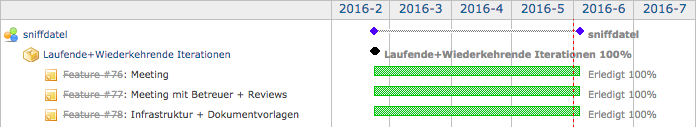
\includegraphics[width=1\textwidth]{./pictures/allgemein.png}\\
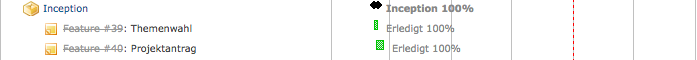
\includegraphics[width=1\textwidth]{./pictures/inception.png}\\
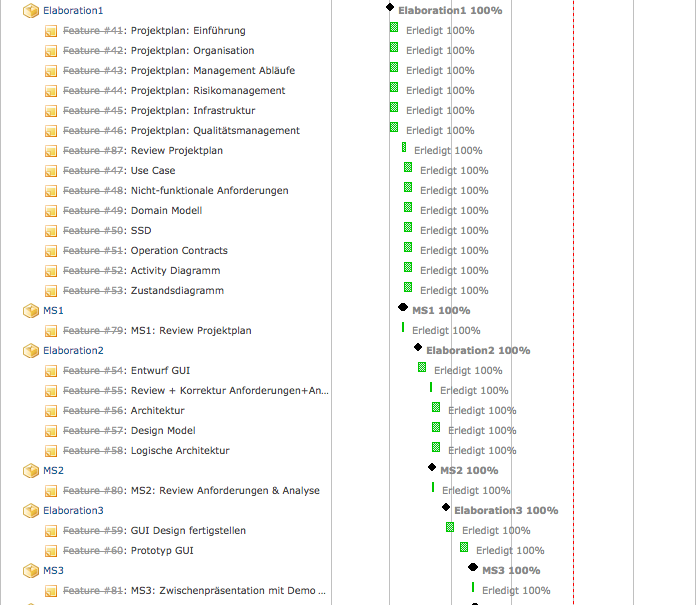
\includegraphics[width=1\textwidth]{./pictures/elaboration.png}\\
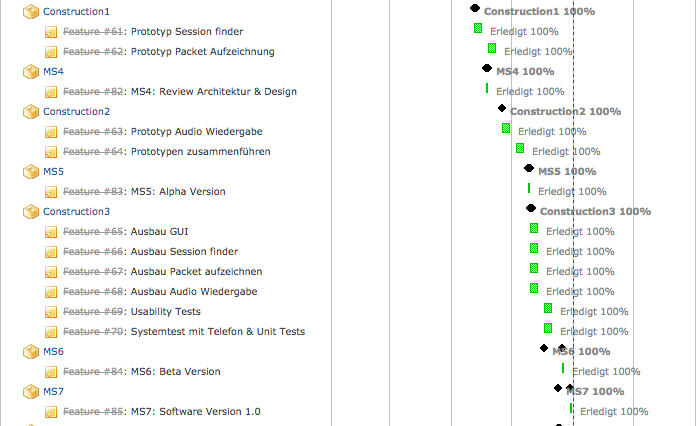
\includegraphics[width=1\textwidth]{./pictures/construction.png}\\
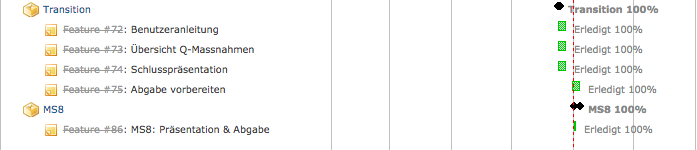
\includegraphics[width=1\textwidth]{./pictures/transition.png}\\

\subsubsection{Geplant vs. Aufgewendet}
Der Projektstart war am Montag den 22. Februar 2016. Die Projektdauer betrug 15 Wochen. 
Wir haben mit einem mindest Wochenaufwand von acht Studen pro Mitglied gereichnet. Bei Problemen oder bei Verzug haben wir mit 12 Stunden pro Woche gerechnet. In der untenstehende Tabelle wird die Auswertung durchgeführt. (Bitte Legende beachten) 
\begin{table}[H]
\centering
    \begin{tabular}{@{} p{2cm} p{1cm} p{1cm} p{1cm} p{1cm} p{1cm} p{1cm} p{1cm} @{}}\toprule    
    {Projekt} & {ZNT} & {ZNTM} & {ZMT} & {ZMTM} & {ZET} & {ZETM} & \textbf{{Diff}}\\ \midrule
    sniffdatel & 480 & 120 & 720 & 180 & 686.00 & 11.43 & \textbf{206} \\ \addlinespace
    \bottomrule
    \end{tabular}
\caption{\textbf{Gesamtzeit}}
\end{table}
\textbf{Legende:}
\begin{itemize}
\item ZNT: Zeitplan Normal Total (15Wx8hx4P)  
\item ZNTM: Zeitplan Normal pro Mitglied Total (15Wx8h)
\item ZMT: Zeitplan Maximum Total (mit 12h statt 8h pro Woche, 15Wx12hx4P) 
\item ZMTM: Zeitplan Maximum Total pro Mitglied (15W*12h)
\item ZET: Zeitplan Effektiv Total 
\item ZETM: Zeitplan Effektiv Total pro Mitglied (ungefähr)
\item Diff: Differenz zur geplanten Zeit (8h pro Woche) 
\end{itemize}
\textit{Wobei W: Woche, P: Personen, h: Stunden.}

\subsubsection{Zeitauswertung pro Mitglied}
\begin{table}[H]
\centering
    \begin{tabular}{@{} p{3cm} p{1.5cm} p{1.5cm} p{1.5cm} p{1.5cm} p{1.5cm} p{1.5cm} @{}}\toprule    
    {Mitglied} & {02-2016} & {03-2016} & {04-2016} & {05-2016} & {06-2016} & {Tot}\\ \midrule
    Giorgio Vincenti & 6.75  & 38.50 & 40.00 & 62.50 & 8.00 & 166.75  \\ \addlinespace
    Andreas Stalder & 7.50 &36.75  & 59.00 & 51.00 & 4.80 & 180.00\\ \addlinespace
    David Meister &  5.50 & 44.50 & 49.00 & 46.50 & 8.00 & 168.50\\ \addlinespace
    Samuel Krieg &  2.25 & 43.00  & 45.50 & 58.00 & 2.00 & 170.75\\ 
    \bottomrule
    \end{tabular}
\caption{\textbf{Zeitauswertung}}
\end{table}

\subsection{Ergebnis}
Zum Schluss der Auswertung zeigen wir zwei Screenshots des Endprodukts. \\
\\
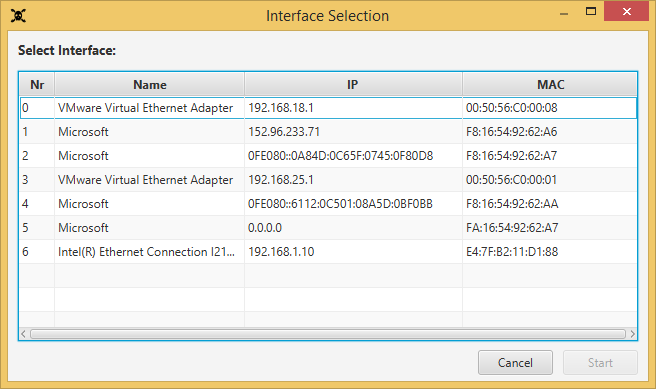
\includegraphics[width=1\textwidth]{./pictures/interface.png}\\
\textit{Screenshot1: sniffdatel während der Interface Auswahl.}\\
\\
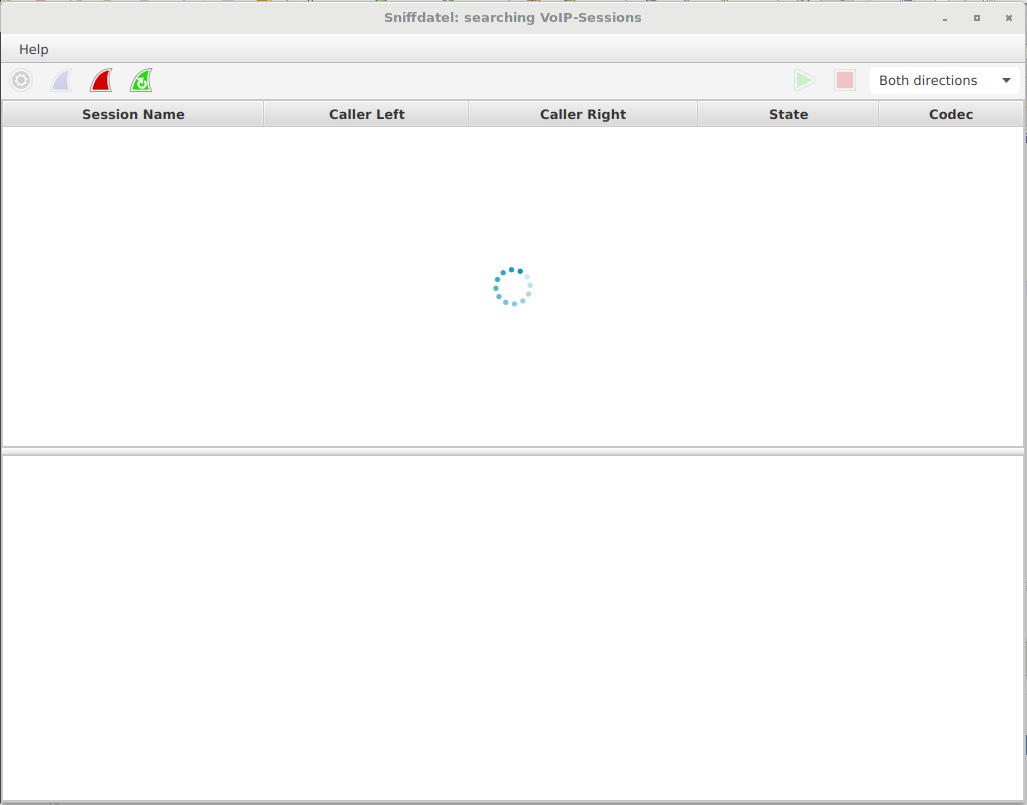
\includegraphics[width=1\textwidth]{./pictures/gui1.png}\\
\textit{Screenshot2: sniffdatel während einem Scanvorgang.}\\
\\
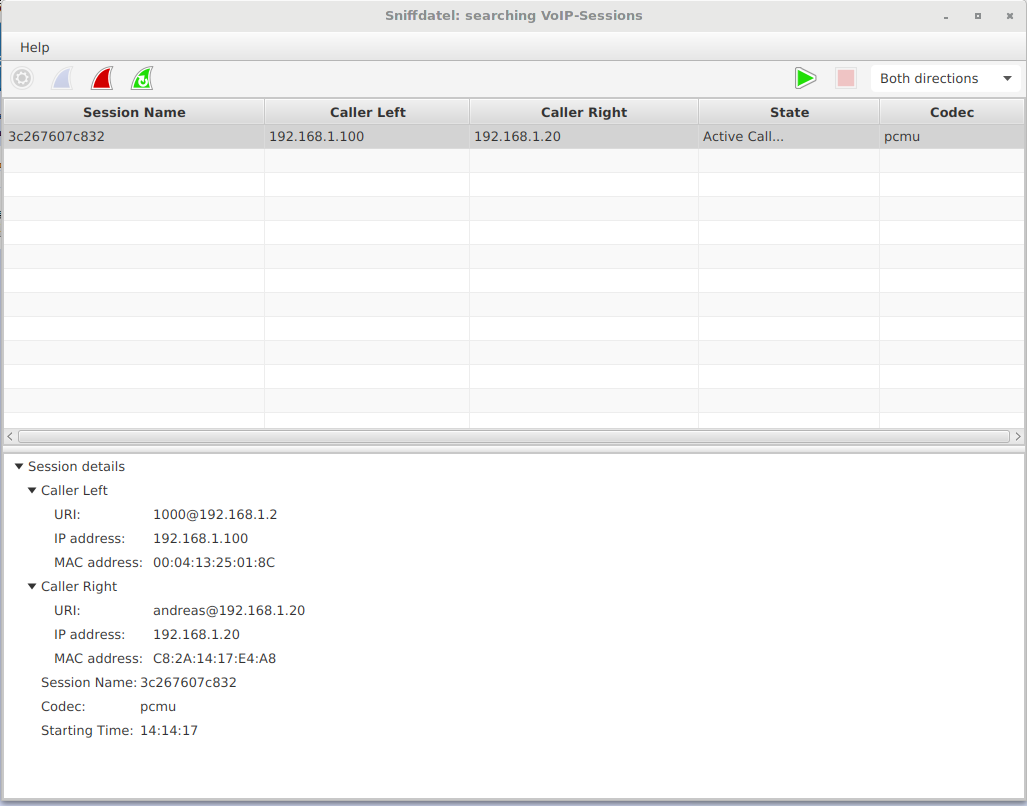
\includegraphics[width=1\textwidth]{./pictures/gui2.png}\\
\textit{Screenshot3: sniffdatel während einem aktiven Anrufs.}\\
\\
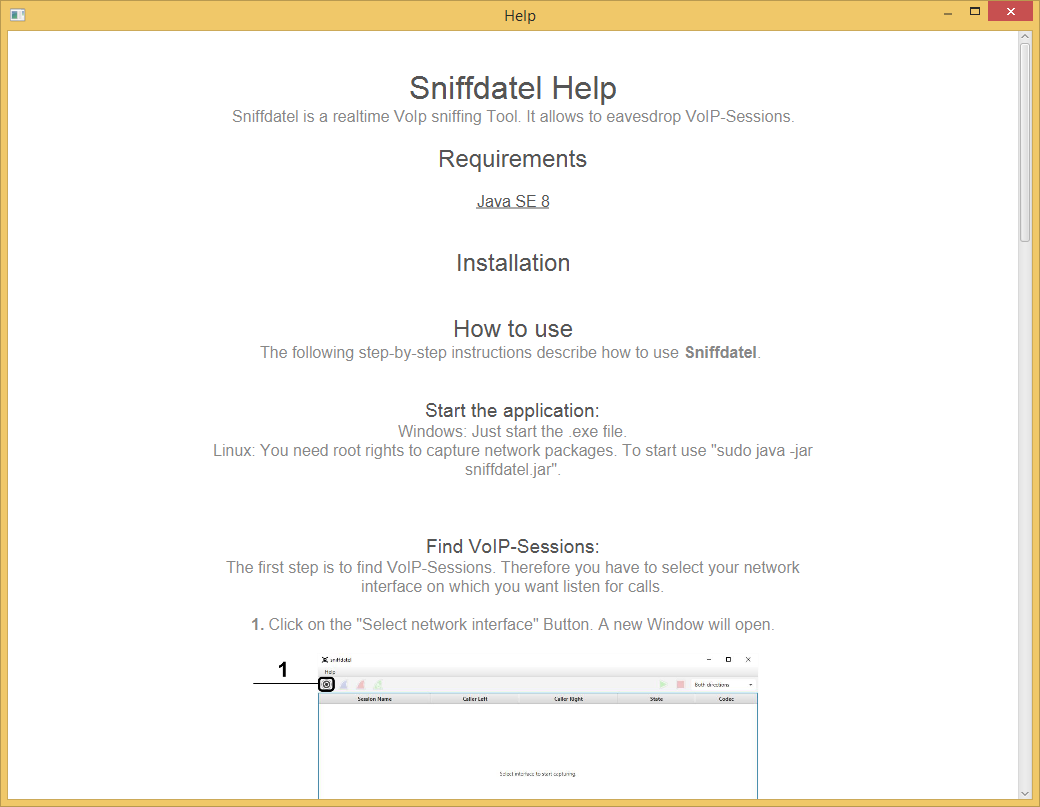
\includegraphics[width=1\textwidth]{./pictures/help.png}\\
\textit{Screenshot4: sniffdatel im Help Menu.}\\
\\
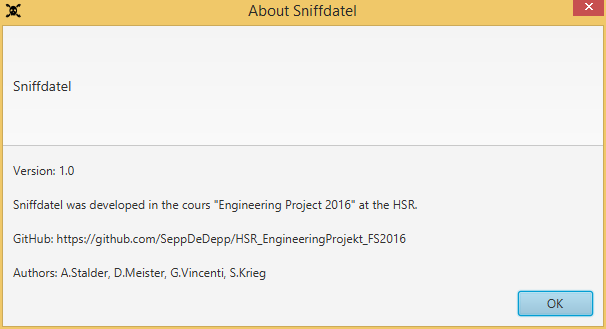
\includegraphics[width=1\textwidth]{./pictures/about.png}\\
\textit{Screenshot5: sniffdatel im About Menu.}\\

\newpage
\section{Erfahrungsberichte}
\subsection{David Meister}
Für mich war das diesjährige Engineering Projekt eine völlig neuartige Erfahrung. Meine Berufserfahrung und meine persönlichen Präferenzen liegen überhaupt nicht im Software Engineering. Ich empfand es als sehr angenehm, die für mich bis anhin sehr theoretischen Software Engineering Grundlagen an einem „richtigen“ Projekt anwenden zu können. Ich konnte nützliche Tools wie git, redmine o.ä. kennenlernen, welche ich noch nicht kannte.\\
\\
Mir gefielen anfangs die ganze Projektplanung und die Anfoderungsspezifikationen respektive deren Dokumentation überhaupt nicht. Auch heute nach dem Projekt fand ich viele Sachen aus der Elaboration Phase unnötig. Vor allem hatte unser Team keine Erfahrungen in der Software Programmierung und den von uns verwendeten Tools, deshalb waren im Nachhinein auch viele Modelle nicht richtig und mussten im Nachhinein geändert werden.\\
\\
Im der Entwicklung des Prototypen nahm das Projekt dann langsam Form an und es wurde uns auch klar, in welche Richtung wir uns bewegen. Die Einarbeit in den verwendeten Frameworks war jedoch riesig und deshalb der Zeitaufwand für 4 ECTS Punkte zu hoch.\\
\\
Ich bin mit dem Endresultat jedoch sehr zufrieden, unsere Software entspricht den gestellten Anforderungen und wir haben ein nützliches Tool zum VoIP Verkehr abhören entwickelt.

\subsection{Giorgio Vincenti}
Es war eine sehr lehrreiche und doch anstregende Zeit. Dank diesem Projekt konnte ich mein erlerntes Wissen im Fach Software Engineering 1 vertiefen und anwenden. Da dies mein erstes Softwareprojekt war, konnte ich ebenfalls viel betreffend Programmierung und Projektmanagement in einem Softwareprojekt erlernen und anwenden. Auch mein Wissen betreffend Git und \LaTeX  konnte ich erfolgreich aufbauen und vertiefen und ich lernte Redmine kennen.\\
\\
Das ausgesuchte Thema \textbf{Realtime VoIP-Sniffer} war besonders interessant, da mein Interesse besonders im der Netzwerkbereich liegt. Dadurch war die Motivation grösser. Ich könnte mir ebenfalls vorstellen das unser Produkt für Schulzwecke genutzt werden könnte. Das würde mich noch viel mehr erfreuen an der Arbeit. \\
\\
Es war sehr schwierig für das Team zu Beginn, da niemand von uns wirklich Programmier- oder Softwareprojekt Erfahrung mit sich bringt. Nach einer gewissen Zeit lief das Projekt jedoch wirklich gut. Die Kommunikation funktionierte einwandfrei und die nötige Infrastruktur wurde von allen produktiv genutzt. Das arbeiten im Team war spannend und ebenfalls lehrreich. Durch das arbeiten im Team war es jedoch schwierig über alles im Bilde zu sein.\\
\\
Rückblickend fand ich den Aufbau der Software sehr spannend, vor dem Programmierbeginn. Ich konnte mir zu Beginn nicht richtig vorstellen wie das Ganze aussieht oder wie das funktionieren soll ohne vorher etwas programmiert zu haben. Es ist beeindruckend wieviel vor der Realisierung erledigt werden muss, und an was alles gedacht werden muss. Das liegt an der mangelnden Praxis Erfahrung. Zum Schluss entstand ein sehr zufriedenstellendes Softwareprodukt welches die definierten Anforderungen erfüllt.\\
\\
Das Arbeiten mit Herr Steffen als Betreuer war sehr angenehem und würde es wieder tun. 

\subsection{Samuel Krieg}
Als Quereinsteiger habe ich mich sehr gefreut auf die erste praktische Programmiererfahrung. Ich fühlte mich oft überfordert. Durch das harmonierende Team und Herrn Steffen hinter uns liess es sich jedoch ertragen. Speziell die erforderten Dokumente stellten ein Problem dar. Der vorhandene Unterrichtsstoff von SE1 und SE2 reichte für mich nicht aus, um die Dokumentation korrekt und seriös zu führen. Wünschenswert wäre ein komplettes Beispielprojekt über diesen Stoff. 
\\
Ich habe den Programmierteil kleiner eingeschätzt. Durch die schlechte Dokumentation der Libraries stellte sich dieser Teil jedoch ebefalls als nicht trivial heraus. Hier half das Arbeiten im Team enorm. Weil meistens alle Teammitglieder vor Ort waren, konnten Probleme durch die geballte Intelligenz meist relativ schnell gelöst werden. 
\\
Ich habe durch das Projekt sehr viel gelernt, manches einfach, anderes auf dem harten Weg. Festgestellt habe ich ebenfalls, dass in der Softwareentwicklung und allgemein in der Informatik das beherrschen der Tools ein sehr zentraler Punkt ist. Der Zeitaufwand war viel zu gross ohne direkte Hilfe. Mein Vorschlag ist, das EngineeringProjekt als Übung in den Modulen SE1 und SE2 durchzuführen.

\subsection{Andreas Stalder}
Nun sind wir mit dem Projekt fertig und ich kann auf eine sehr interessante Zeit zurückblicken. Ich durfte noch nie bei einem so grossen Projekt mitarbeiten. Durch dieses Projekt sieht man sehr gut, dass der gelernte Stoff vom Fach Software Engineering 1 sehr wichtig ist. Ohne dieses Wissen wäre das Projekt wohl nicht zu Stande gekommen. Man sieht nun endlich für was dies alles ist und lernt es zu schätzen, da die gezeigten Tools und Verfahren die täglichen Arbeiten unterstützen.\\
\\
Die Arbeit im Team war sehr gut. Wir konnten offen alles ansprechen und über die Probleme diskutieren. So waren viele Probleme schnell gelöst und wir könnten wieder weiterarbeiten. Durch die kollegiale Arbeitsweise, machte es immer wieder Spass am Projekt weiter zu arbeiten.\\
\\
Das Thema emfpand ich als sehr spannend. Da wird in mehreren Modulen mit VoIP zu tun hatten, konnten wir so das Thema noch vertiefen und verstehen nun diese Technologie sehr gut. Dies wird mir sicher auch im Berufs-  oder im Privatleben weiterhelfen, da VoIP die Zukunft ist. \\
\newpage

\section{Eigenständigkeitserklärung}

Wir erklären hiermit, 
\begin{itemize}
\item dass wir die vorliegende Arbeit selber und ohne fremde Hilfe durchgeführt haben, ausser derjenigen, welche explizit erwähnt ist,
\item dass wir sämtliche verwendeten Quellen erwähnt und gemäss gängigen wissenschaftlichen Zitierregeln korrekt angegeben haben und
\item dass die Urheberschaft aller Arbeitsergebnisse korrekt angegeben ist.
\end{itemize}

\noindent \textbf{Name, Unterschrift:} 
\\
\\
Giorgio Vincenti\\

\includegraphics[width=0.2\textwidth]{./pictures/gv.png}\\
David Meister\\

\includegraphics[width=0.2\textwidth]{./pictures/dm.png}\\
Andreas Stalder\\

\includegraphics[width=0.2\textwidth]{./pictures/as.png}\\
Samuel Krieg\\

\includegraphics[width=0.2\textwidth]{./pictures/sk.png}\\
\textbf{Ort, Datum:} Rapperswil den 31. Mai 2016 
\end{document}

